\chapter{Beschreibung d. Motorseglers, seiner Systeme und Anlagen}

\section{Einführung}
Der vorliegende Abschnitt enthält eine Beschreibung des Motorsegelflugzeuges sowie seiner Systeme und Anlagen mit Benutzungshinweisen. 

\section{Bedienorgane}
Jeder Sitz ist ausgestattet mit Steuerknüppel, Seitenruderpedalen, Brems- und Wölbklappenhebel (jeweils links) und Ausklinkknopf (zwischen den Beinen).\\
Haubenverriegelung: Bedienhebel im Instrumentenpilz.\\
Haubennotabwurf: Zusätzlich zum Bedienhebel im Instrumentenpilz den roten Griff dahinter ziehen.\\
Die Bremse ist mit der Bremsklappe gekoppelt und wird im hinteren Bereich der Bremsklappen mit betätigt.\\
Die Trimmung ist in der Mittelkonsole angeordnet. Die Betätigung erfolgt durch Ziehen nach links und verschieben des Hebels (Rastung durch Federkraft).\\
Die Lüftung befindet sich links und rechts neben den Sitzen. Die Betätigung erfolgt durch Entriegeln,  ziehen nach hinten und verriegeln\\


\section{Fahrwerk}
Der Bedienhebel für das Fahrwerk befindet sich in der Mittelkonsole und wird durch umlegen des Hebels betätigt.\\
Beim Einfahren des Fahrwerkes empfiehlt es sich, den Hebel in einem Zug nach hinten durch zu ziehen.\\
Zum Ausfahren des Fahrwerkes den Hebel aus der Verknieung drücken, Hebel dann langsam nach vorn führen um ein durchschlagen zu verhindern und in vordere Verknieung drücken.\\
Die hydraulische Doppelscheibenbremse wird mit vollständigem Ausfahren der Bremsklappen mitbetätigt und ist gut wirksam.


\section{Instrumentierung}
Im Instrumentenpilz (Abb. 6.1) sind die Instrumente zur Flugüberwachung (Fahrtmesser mit Meßbereich mindestens $50 \frac{km}{h}$ bis $300 \frac{km}{h}$ ,Höhenmesser, Variometer), Funksprechgeräte und Navigationsgeräte angeordnet.

\begin{figure}[ht]
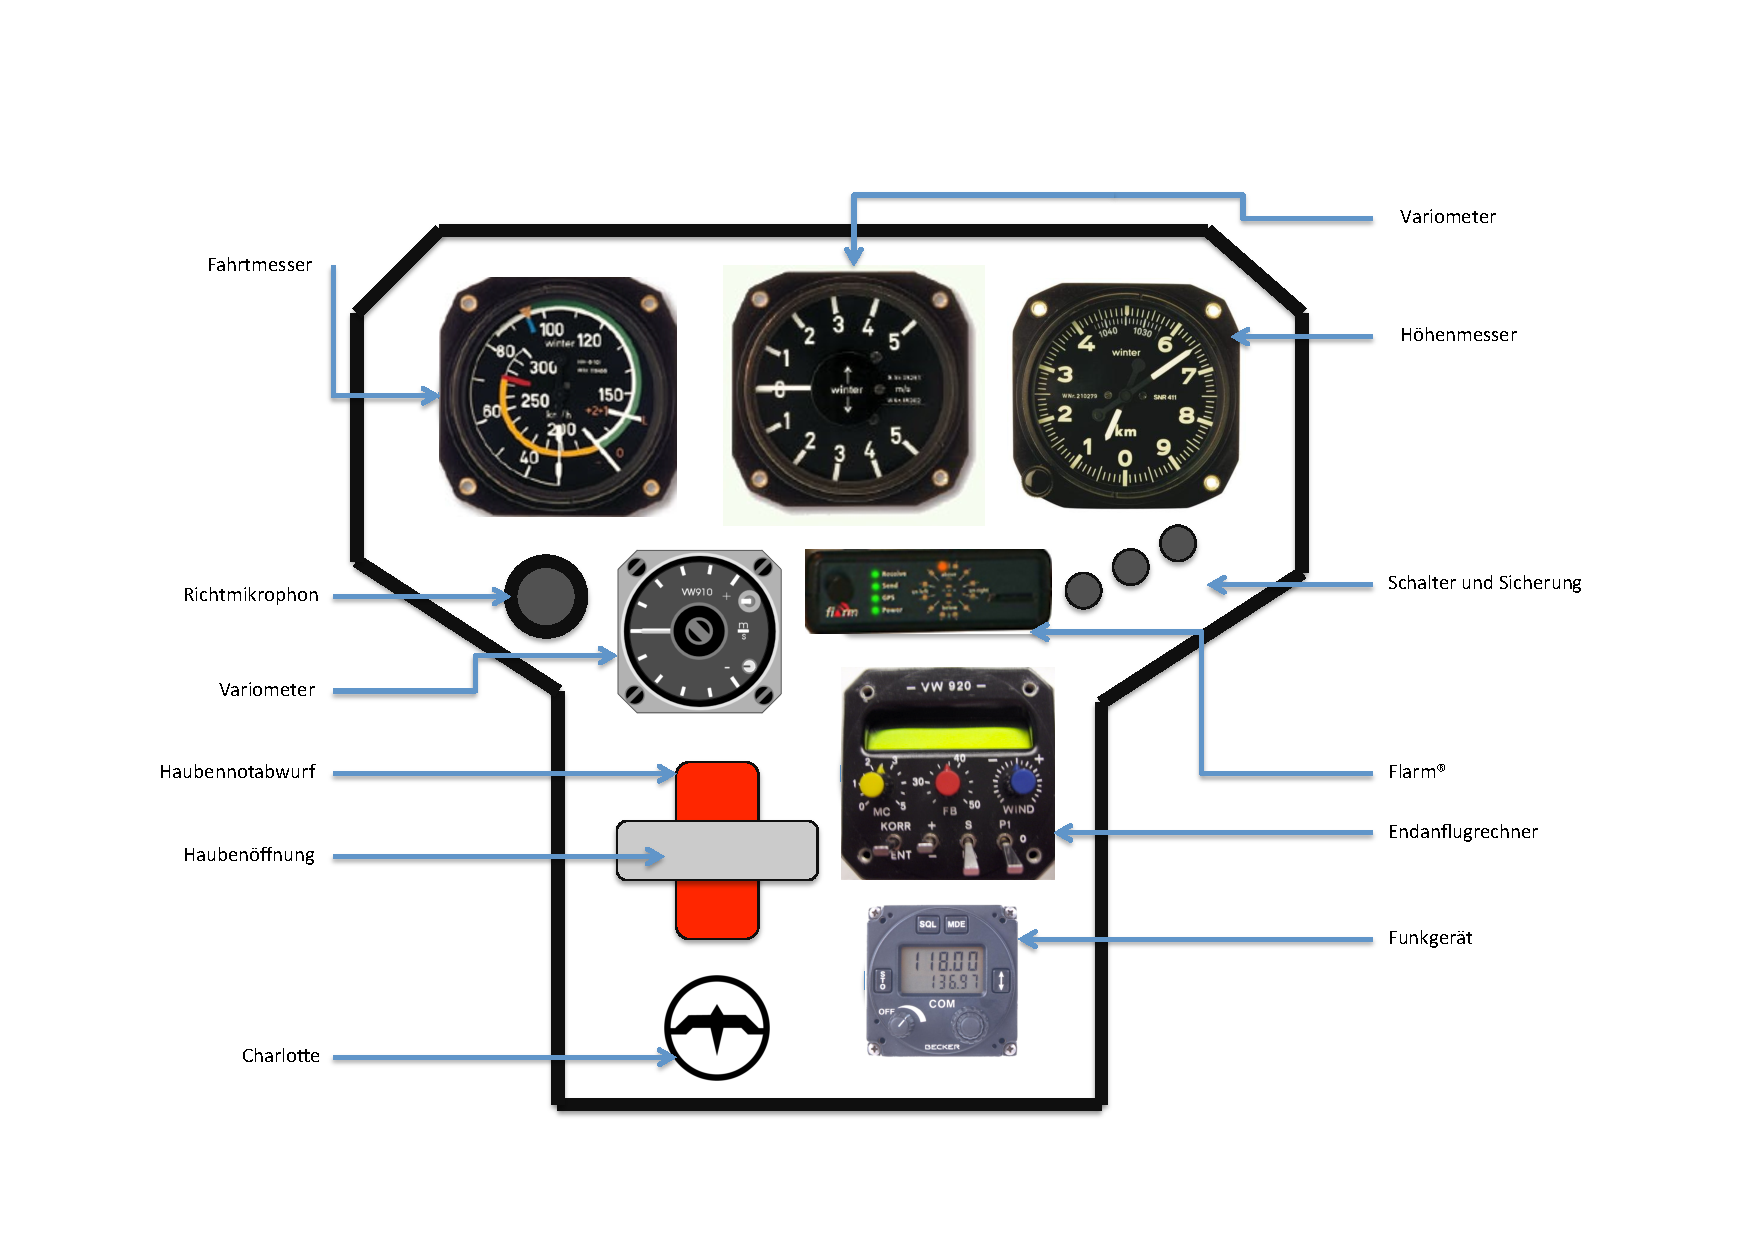
\includegraphics[angle=90,width=\textwidth]{bilder/instrumentenpilz.pdf}
\caption{Instrumentenpilz}
\end{figure}

\section{Bremsklappen}
Doppelstöckige Schempp-Hirth Bremsklappen auf der Oberseite des Innentragflügels. Der Antrieb mit Verknieung ist im Mittelrumpf angeordnet.

\section{Gepäckraum}
Das Gepäckfach befindet sich hinter dem rechten Piloten und hat eine maximale Zuladung von $10kg$.

\newpage
\section{Triebwerksanlage}
nicht eingebaut

\newpage
\section{Faltpropeller}
nicht eingebaut